\chapter{Hardware Documentation}

\begin{figure}[H]
	\centering
	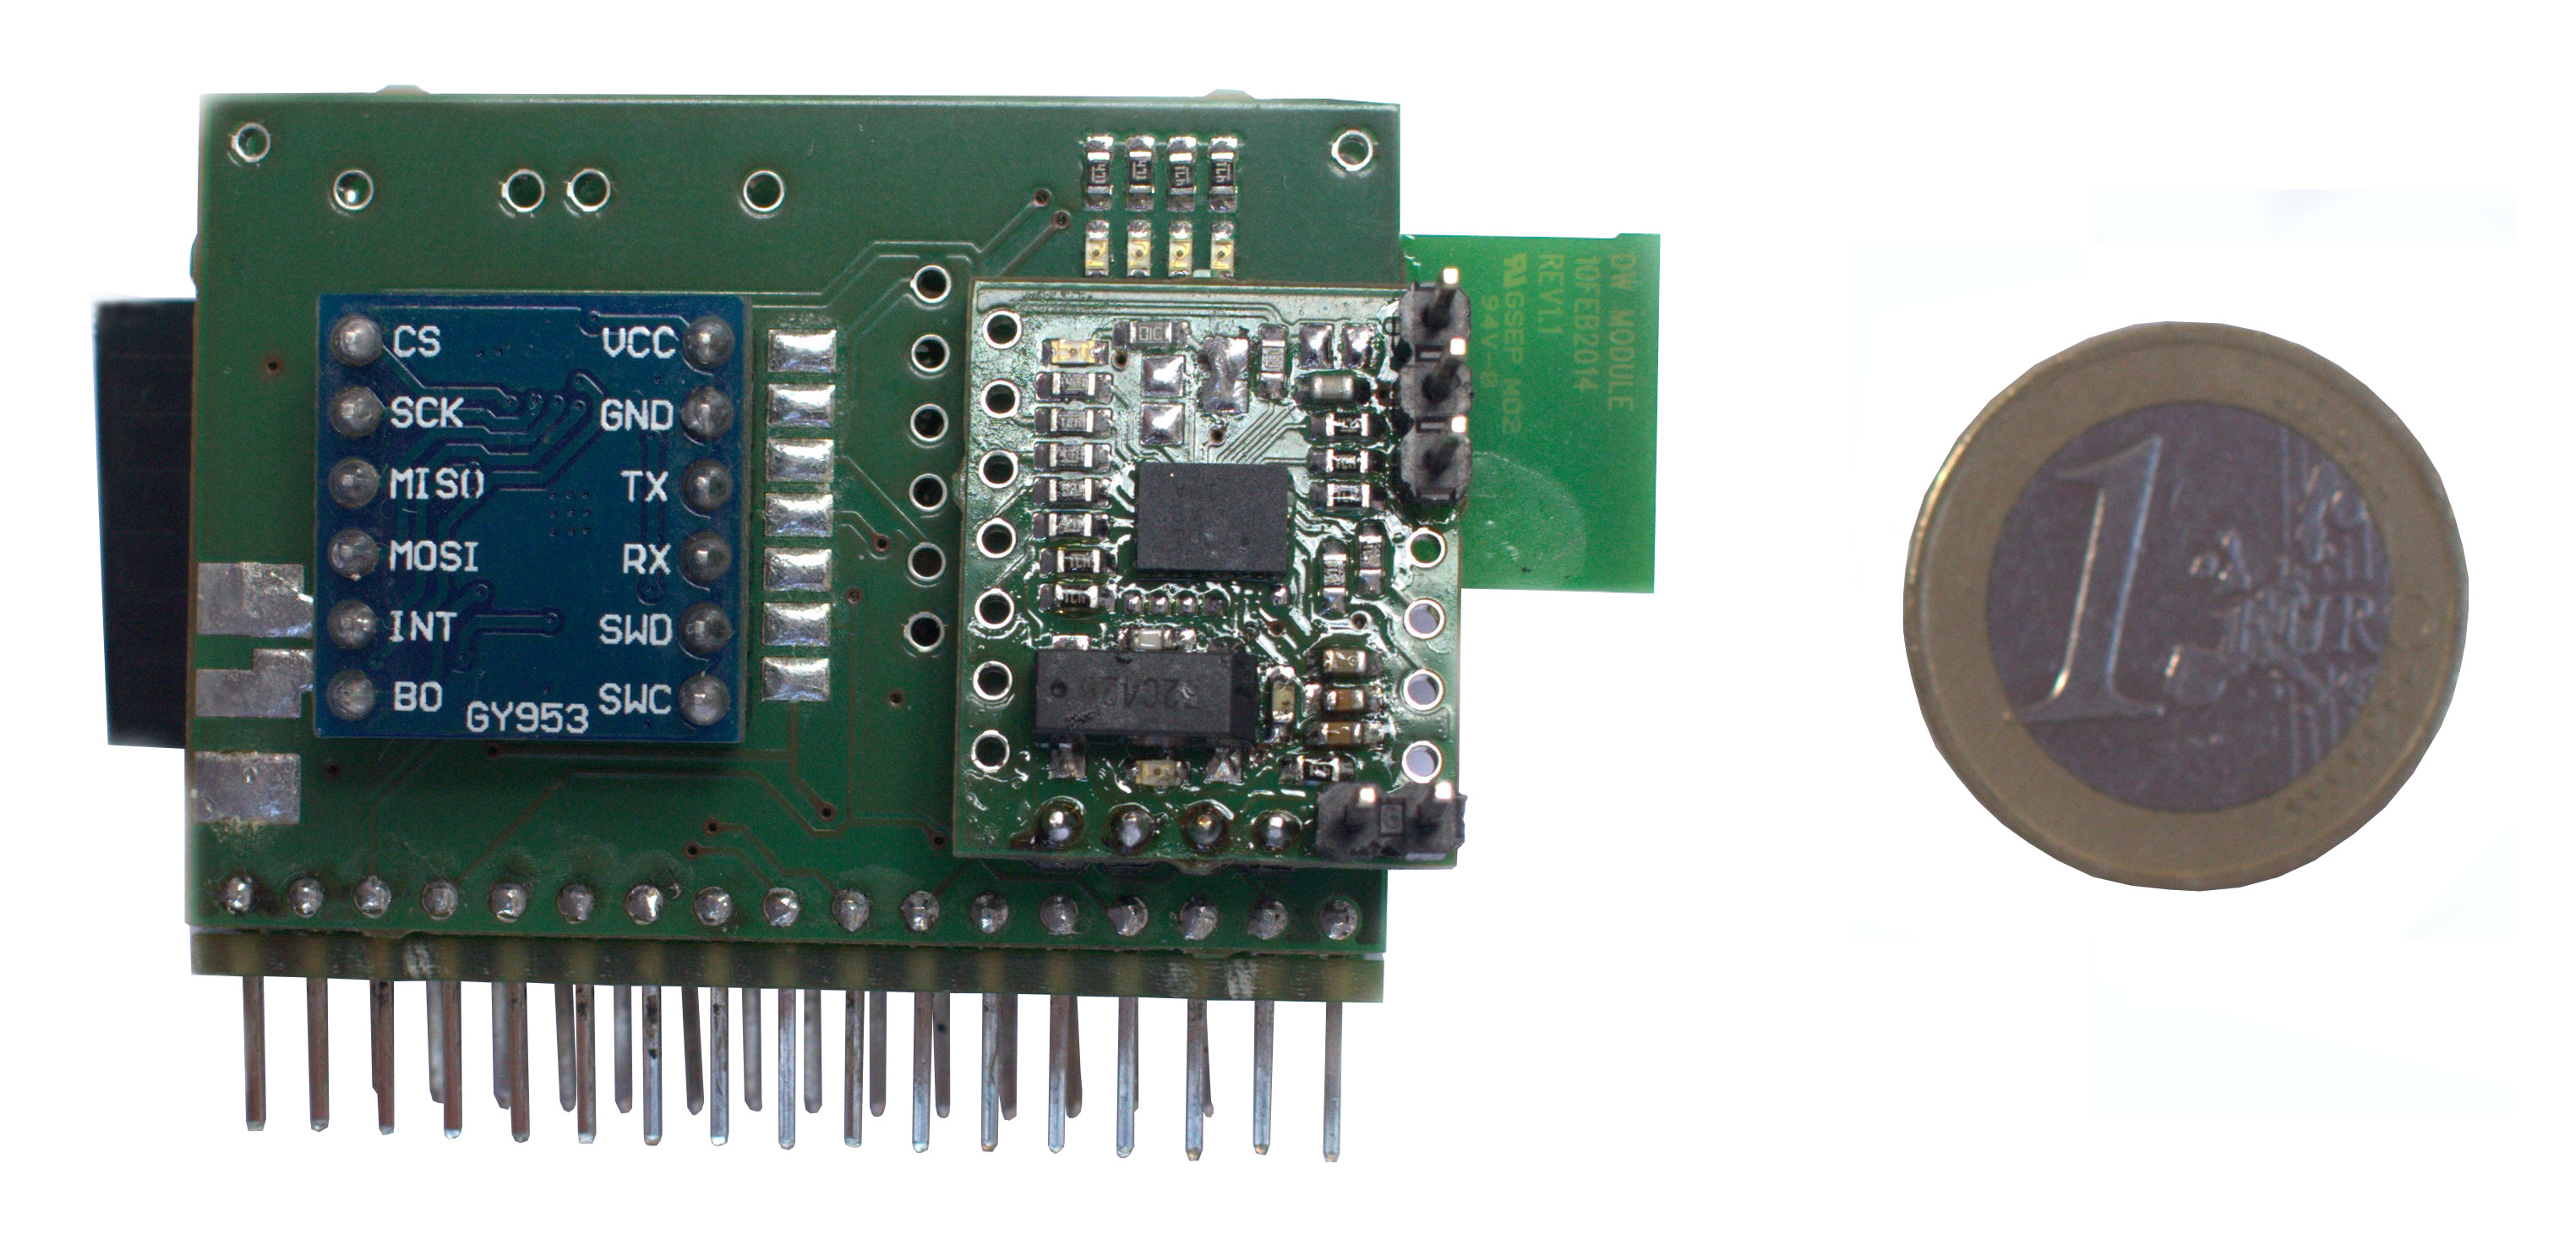
\includegraphics[width=16cm]{img/HWassembled.jpg}
	\label{HWassembled}
	\caption{Assembled Sensor Board prototype}
\end{figure}

\section{Overview}
Sensor Board is a prototype of autonomous hardware platform with microprocessor and various inertial, atmospheric and navigation sensors. The device can be used in many cases from logging data to movement control. The prototype works fully autonomously without connection to external power supply or other electronics, but allows wireless or wired connection to other electronic devices.

\subsection{Features}
\begin{itemize}
	\setlength\itemsep{0.2em}
	\item[--] No external power supply needed
	\item[--] Internal rechargeable battery
	\item[--] Charging from USB or any \SI{5}{V} source
	\item[--] Allowed simultaneous connection to USB and other power supply
	\item[--] Three different triaxial acceleromemers, dynamic gyroscopes and two different triaxial magnetometers
	\item[--] Barometer, light sensor, air humidity, temperature
	\item[--] A/D converters for connecting external sensors
	\item[--] TDOA location system with \SI{10}{cm} precission in \SI{300}{m} radius
	\item[--] External UART connector for GPS or radio communication
	\item[--] Hybrid WiFi and Bluetooth
	\item[--] Servo outputs and connector with other peripheries
	\item[--] User programmable dual core ESP32 processor
	\item[--] Various sleep modes to save battery power
	\item[--] More than 10 hours of operation from battery
	\item[--] Buttons and LEDs for interaction with user
	\item[--] Micro SD card up to \SI{32}{GB} for logging data (accessible from user program)
	\item[--] ARM Cortex-M0 co-processor for computing (sensor fusion, data analysis)
\end{itemize}

\subsection{Properties}

\begin{table}[H]
	\centering
	\begin{tabular}{|l|c|c|}
		\hline
		Parameter & Value & Unit \\
		\hline \hline
		Dimensions & 60 $\cdot$ 31 $\cdot$ 13 & mm \\
		Min Voltage & $-0.5$ & V \\
		Max Voltage & $5.5$ & V \\
		Max current & $2.1$ & A \\
		Max battery life & $12$ & hours \\
		WiFi antenna range & $10$ & m \\
		Bluetooth antenna range & $10$ & m \\
		TDOA location precission & $10$ & cm \\
		TDOA location range & $300$ & m \\
		Average charging time & $60$ & minutes \\
		Min temperature & $-10$ & \degreeCelsius \\
		Max temperature & $80$ & \degreeCelsius \\
		\hline
	\end{tabular}
	\caption{Properties}
	\label{HWmaxRatings}
\end{table}

\section{Getting Started}

\subsection{Assembling}
The device is assembled from three parts, two sandwich boards and one connector board. Optional devices like BMF055 board, GY953, HM-TRP or GPS can be connected to prepared ports. The parts are shown in figure \ref{HWassembling}.

\begin{figure}[H]
	\centering
	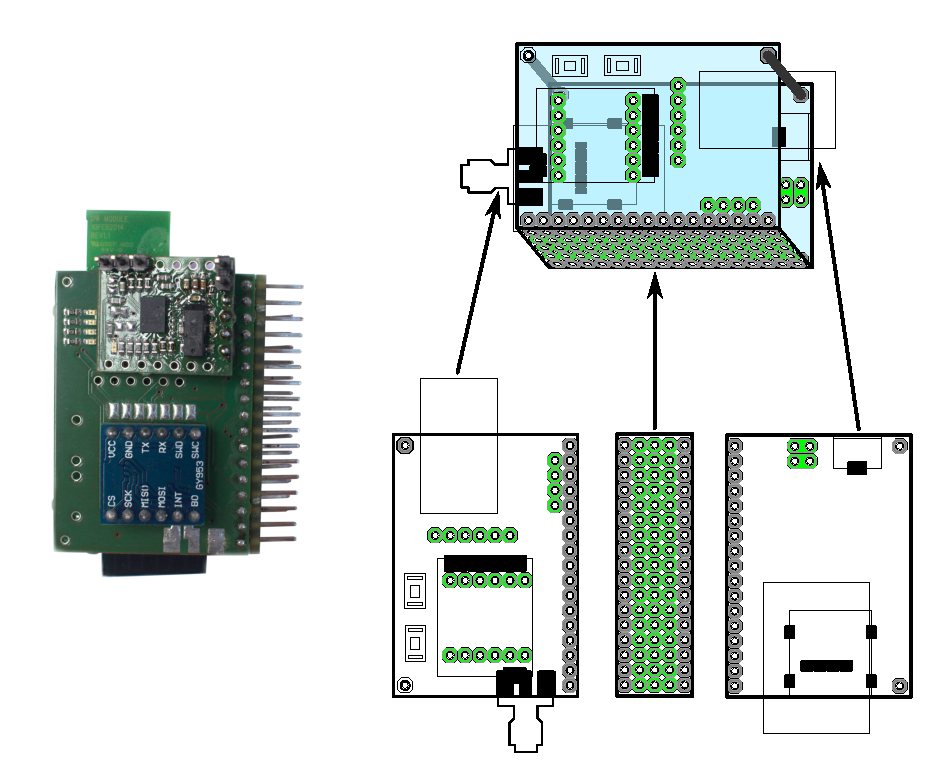
\includegraphics[scale=1]{img/assemblingHW.pdf}
	\label{HWassembling}
	\caption{Assembling the Sensor Board prototype}
\end{figure}

\subsection{Components Description}

\begin{figure}[H]
	\centering
	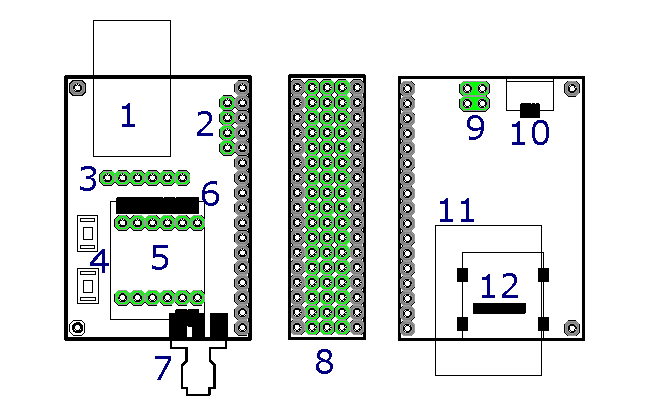
\includegraphics[scale=1]{img/componentsDescription.pdf}
	\label{HWcomponents}
	\caption{Components of the Sensor Board}
\end{figure}

\begin{table}[H]
	\centering
	\begin{tabular}{|c|l|c|}
		\hline
		Number & Description & Datasheet\\
		\hline \hline
		1 & DWM1000 location sensor & //todo \\
		2 & BMF055 board connector (UART) & //todo \\
		3 & HM-TRP 433/868 MHz radio connector & //todo \\
		4 & Software buttons & N/A \\
		5 & GY-953 connector & //todo \\
		6 & HM-TRP 433/868 MHz radio SMD pads & //todo \\
		7 & RPSMA antenna connector for HM-TRP radio & //todo \\
		8 & External pins & Section \ref{pinNumbering} \\
		9 & Battery connector & Section \ref{pinNumbering} \\
		10 & Micro USB connector & //todo \\
		11 & ESP-WROOM-32 with WiFi/Bluetooth antenna & //todo \\
		12 & Micro SD card slot & //todo \\
		\hline
	\end{tabular}
	\caption{Description of components of the Sensor Board}
	\label{table:componentsDescription}
\end{table}

\section{Pin Connections}

\subsection{Pin Numbering}
\label{pinNumbering}

\begin{figure}[H]
	\centering
	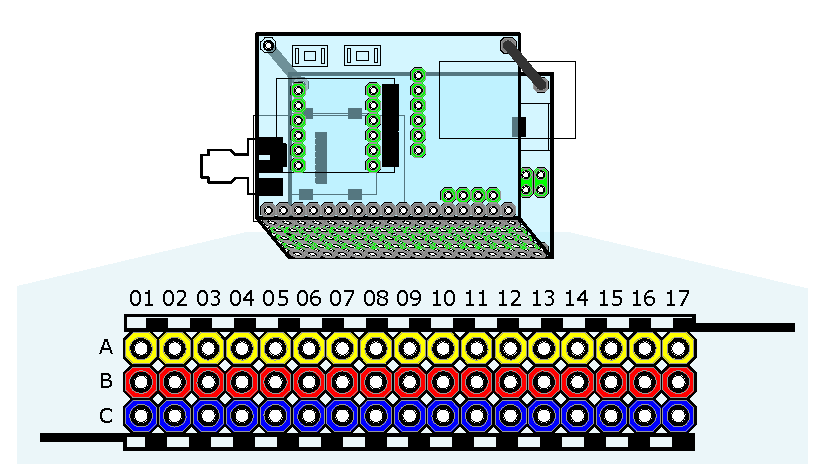
\includegraphics[scale=1]{img/externalPins.pdf}
	\caption{External pins numbering}
	\label{fig:externalPins}
\end{figure}

\begin{table}[H]
	\centering
	\begin{tabular}{|c||c|c|c|c|c|c|c|c|}
		\hline
		& 01 & 02 & 03 & 04 & 05 & 06 & 07 & 08 \\
		\hline \hline
		A & GND & +3V3 & SENSOR\_VP & SENSOR\_VN & IO33 & IO25 & IO32 & IO26 \\
		B & \multicolumn{8}{|c|}{Pins B01 -- B17 internally connected, details in section \ref{jumpersExternalPins}} \\
		C & \multicolumn{8}{|c|}{GND} \\
		\hline
	\end{tabular}

	\vspace{0.5cm}
	
	\begin{tabular}{|c||c|c|c|c|c|c|c|c|c|c|}
		\hline
		& 09 & 10 & 11 & 12 & 13 & 14 & 15 & 16 & 17 & \\
		\hline \hline
		A & IO18 & IO19 & IO21 & IO16 & IO17 & IO23 & IO22 & IO27 & +5V & \\
		B & \multicolumn{10}{|c|}{Pins B01 -- B17 internally connected, details in section \ref{jumpersExternalPins}} \\
		C & \multicolumn{10}{|c|}{GND} \\
		\hline
	\end{tabular}
	\caption{External pins mapping}
	\label{tab:externalPins}
\end{table}

\begin{table}[H]
	\centering
	\begin{tabular}{|c|c|c|c|c|c|}
		\hline
		Number & Name & Safety resistor & Pull-up & Device & Pin \\
		\hline \hline
		01 & GND & N/A & N/A & N/A & N/A \\
		02 & +3V3 & N/A & N/A & N/A & N/A \\
		03 & RADIO\_RX & Yes & No & ESP32 & SENSOR\_VP \\
		04 & RADIO\_TX & Yes & No & ESP32 & SENSOR\_VN \\
		05 & BTN1 & No & Yes & ESP32 & IO33 \\
		06 & BTN0 & No & Yes & ESP32 & IO25 \\
		07 & LED4 & Yes & No & ESP32 & IO32 \\
		08 & SCL0 & Yes & Yes & ESP32 & IO26 \\
		09 & SCK0 & Yes & No & ESP32 & IO18 \\
		10 & MISO0 & Yes & No & ESP32 & IO19 \\
		11 & MOSI0 & Yes & No & ESP32 & IO21 \\
		12 & MPU\_TX & Yes & No & ESP32 & IO16 \\
		13 & MPU\_RX & Yes & No & ESP32 & IO17 \\
		14 & CS\_DECA & Yes & No & ESP32 & IO23 \\
		15 & CS\_MPU2 & Yes & No & ESP32 & IO22 \\
		16 & SDA0 & Yes & No & ESP32 & IO27 \\
		17 & +5V & N/A & N/A & N/A & N/A \\
		\hline
	\end{tabular}
	\caption{External pins properties}
	\label{tab:externalPinsProperties}
\end{table}

\paragraph{Note:} Some external pins are not connected only to processor, but they are connected to other chips in parallel. The other chips are connected only via input only pins or with safety resistor. So, the possibility of damage by incorrect connection or by wrong software is minimized.

\subsection{Pin Description}
\begin{itemize}
	\item 01 -- \textbf{GND}: Ground
	\item 02 -- \textbf{+3V3}: Power Supply \SI{+3.3}{V} from linear stabilizer
	\item 03 -- \textbf{RADIO\_RX}: UART receive pin for external devices like radio communication or GPS
	\item 04 -- \textbf{RADIO\_TX}: UART transmit pin for external devices like radio communication or GPS
	\item 05 -- \textbf{BTN1}: Usage defined by user software, internally connected to button 1
	\item 06 -- \textbf{BTN0}: Usage defined by user software, internally connected to button 0
	\item 07 -- \textbf{LED4}: Usage defined by user software, internally connected to LED4
	\item 08 -- \textbf{SCL0}: \itwoc clock pin for external devices, internally connected to sensors
	\item 09 -- \textbf{SCK0}: SPI clock pin for external devices, internally connected to sensors
	\item 10 -- \textbf{MISO0}: SPI data output pin for external devices, internally connected to sensors
	\item 11 -- \textbf{MOSI0}: SPI data input pin for external devices, internally connected to sensors
	\item 12 -- \textbf{MPU\_TX}: UART transmit pin for GY953 or external device
	\item 13 -- \textbf{MPU\_RX}: UART receive pin for GY953 or external device
	\item 14 -- \textbf{CS\_DECA}: Usage defined by user software, internally used as chip select pin for DWM1000 TDOA location sensor
	\item 15 -- \textbf{CS\_MPU2}: Usage defined by user software, internally connected to GY953 port
	\item 16 -- \textbf{SDA0}: \itwoc data pin for external devices, internally connected to sensors
	\item 17 -- \textbf{+5V}: \SI{+5}{V} power supply from battery or USB or external source, the battery voltage is converted to \SI{5}{V}
\end{itemize}

\paragraph{Note:} All pins except power supply pins can be redefined by software. Their new definition shouldn't be in collision with other connected parts. For details see figures \ref{sch1} and \ref{sch2}.

\subsection{Power Supply}
\label{jumpersExternalPins}
The pins B01 -- B17 are defined by jumpers. We usually need these pins connected to power supply. We can define the voltage by connecting arbitrary B pin to target power supply. The pins B01 -- B17 are internally connected, but they are not connected to anything else. We can define pins B01 -- 17 as:
\begin{itemize}
	\item \textbf{GND} by connecting A01 and B01 by jumper
	\item \textbf{+3V3} by connecting A02 and B02 by jumper
	\item \textbf{+5V} by connecting A17 and B17 by jumper
	\item \textbf{anything} by connecting any B pin to our target
\end{itemize}

\begin{figure}[H]
	\centering
	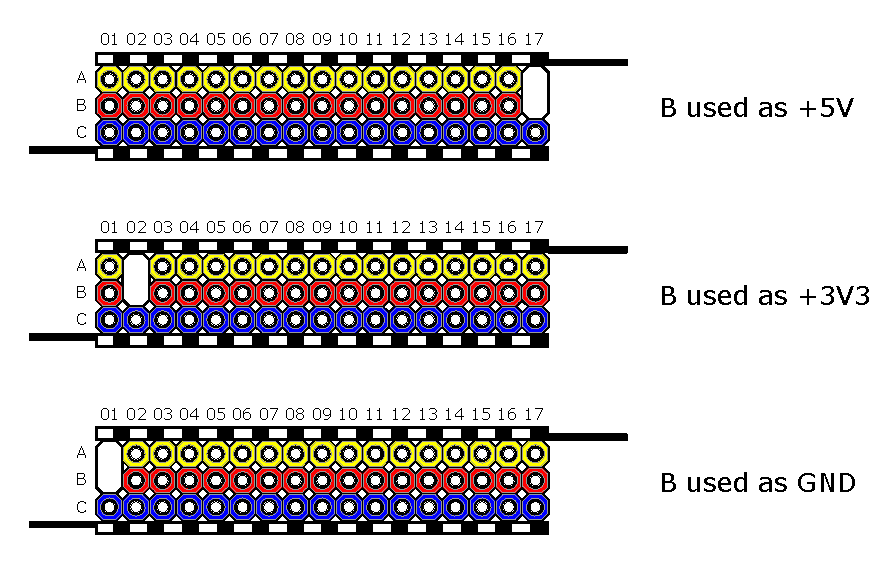
\includegraphics[scale=1]{img/jumpers.pdf}
	\caption{Power supply definition by jumpers}
	\label{fig:jumpersSupply}
\end{figure}

\section{LED Meanings}

\begin{figure}[H]
	\centering
	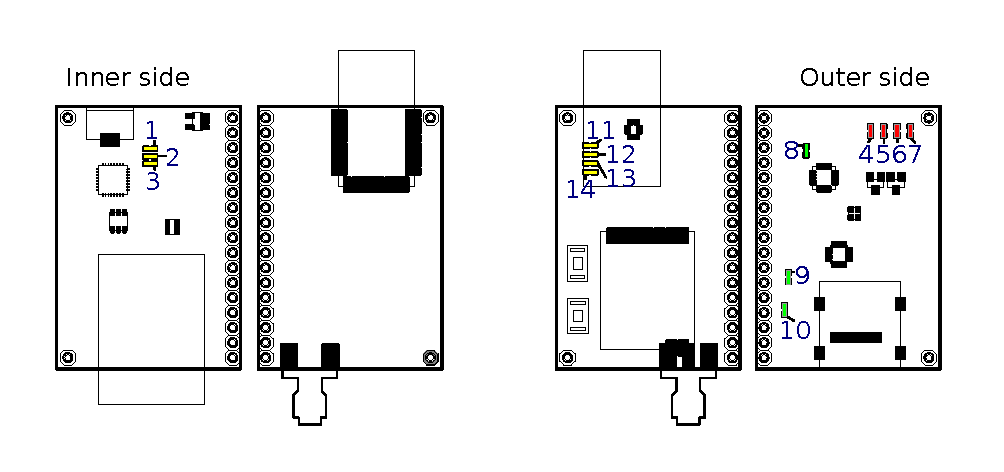
\includegraphics[scale=1]{img/LEDmeanings.pdf}
	\caption{Sensor Board LED meanings}
	\label{fig:LEDmeaning}
\end{figure}

\begin{enumerate}
	\item \textbf{LED\_CBUS3}: (yellow) FTDI LED \cite{FTDI}, USB power indication
	\item \textbf{LED\_CBUS2}: (yellow) FTDI LED \cite{FTDI}, USB connection indication
	\item \textbf{LED\_CBUS4}: (yellow) FTDI LED \cite{FTDI}, USB data transfer indication
	\item \textbf{LED\_5V}: (red) \SI{5}{V} power LED
	\item \textbf{LED\_3V3}: (red) \SI{3.3}{V} power LED
	\item \textbf{LED\_VCCIO}: (red) VCCIO power LED
	\item \textbf{LED\_USB}: (red) USB power LED
	\item \textbf{LED6}: (green) Charging the battery indication
	\item \textbf{LED4}: (green) Software configurable LED
	\item \textbf{LED5}: (green) Software configurable LED
	\item \textbf{LED7}: (yellow) DWM1000 TXLED \cite{DWM1000}
	\item \textbf{LED3}: (yellow) DWM1000 RXLED \cite{DWM1000}
	\item \textbf{LED2}: (yellow) DWM1000 SFDLED \cite{DWM1000}
	\item \textbf{LED1}: (yellow) DWM1000 RXOKLED \cite{DWM1000}
\end{enumerate}

\section{Internal Connections}

\subsection{Internal Pins}
//todo

\begin{figure}[H]
	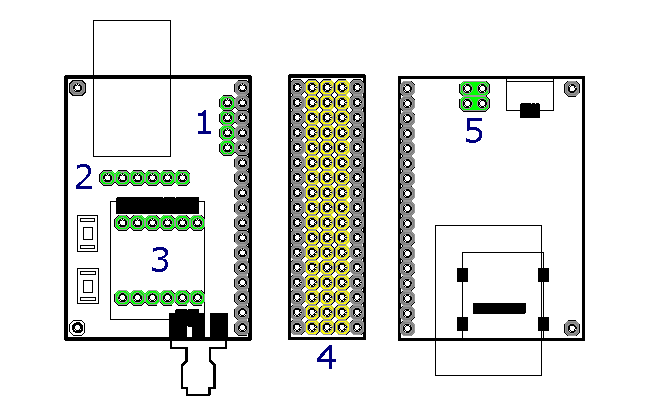
\includegraphics[scale=1]{img/pinSections.pdf}
\end{figure}

\begin{table}[H]
	\begin{tabular}{|c|c|l|}
		\hline
		Number & Usage & Description \\
		\hline
		1 & Internal & BMF055 board connector (UART) \\
		2 & Internal & HM-TRP 433/868 MHz radio connector \\
		3 & Internal & GY-953 connector \\
		4 & External & External pins \\
		5 & Internal & Battery connector \\
		\hline
	\end{tabular}
\end{table}

//todo: detaily ke kazdemu

\subsubsection{BMF055 board connector (UART)}
\subsubsection{HM-TRP 433/868 MHz radio connector}
\subsubsection{GY-953 connector}
\subsubsection{External pins} \ref{pinNumbering}
\subsubsection{Battery connector}

//todo: vyznam testpadu

\section{BMF055 Extension Board}
//todo

\subsection{Pin Connection}
//todo

\subsection{LED Meanings}
//todo



\section{Sensor Board Drawings}
//todo: pridat vedle sebe fotku, render, nakres a eagle brd
